\subsection{Реберные раскраски}

$C$ --- множество цветов

\begin{defn}
    
    Реберная раскраска: $c: E \to C$(красим ребра).
\end{defn}

\begin{defn}

    Раскраска $c$ правильная, если $c(e) \neq c(e')$ для всяких смежных ребер $e, e'$.
    \begin{center}
        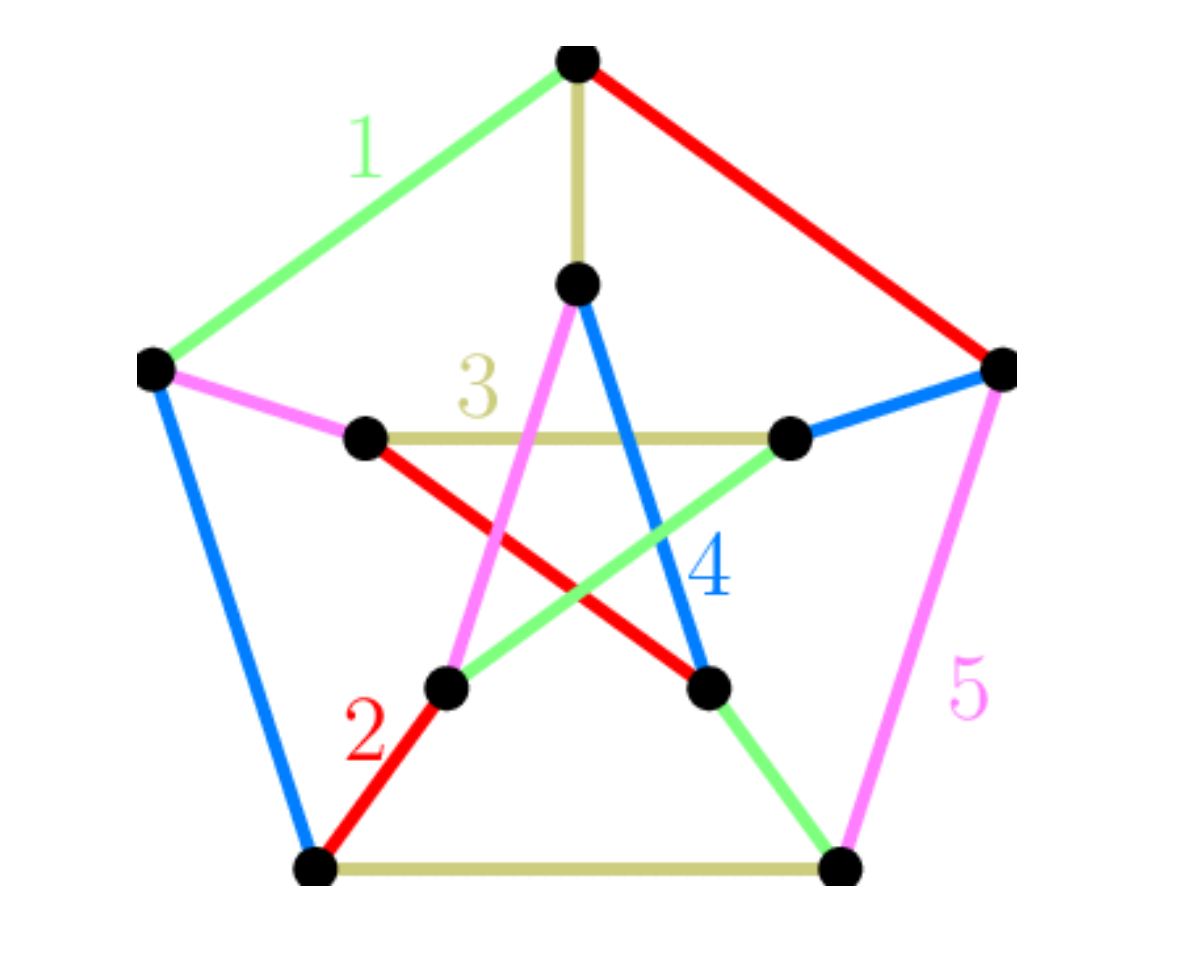
\includegraphics[width=0.5\textwidth]{par41edgecol.png}
    \end{center}
    
    Иными словами, для каждого цвета множество ребер, раскрашенных в данный цвет, это паросочетание.
\end{defn}

\begin{theorem}[Кенига о раскаске ребер]
    В двудольном графе $G = (V_1, V_2, E)$ существует правильная раскраска ребер в $D$ цветов, где $D$ --- наибольшая степень вершины.
\end{theorem}

\begin{proof}

    Индукция по наименьшей степени вершины $d$, от больших к меньшим.

    \textsl{База:} $d = D$, то есть $D$-регулярный граф.

    Покажем, что он удовлетворяет условию теорему Холла:
    \begin{itemize}
        \item всякое множество $U_1 \subseteq V_1$ соединено со своими соседками из $V_2$ ровно $D|U_1|$ ребрами
        
        \item так как у каждой соседки степень тоже $D$, этих соседок всего не менее чем $\frac{D|U_1|}{D} = |U_1|$.
    \end{itemize}

    По теореме Холла есть совершенное паросочетание.

    Удаляем ребра паросочетания, остается $(D - 1)$-регулярный двудольный граф, в нем опять есть совершенное паросочетание, и.т.д.

    Полученные $D$ непересекающихся паросочетаний образуют искомую раскраску ребер $G$.

    \textsl{Переход:} $d < D$. Пусть $G = (V_1, V_2, E)$ --- граф.

    \begin{itemize}
        \item Строим копию этого графа: $G' = (V_1', V_2', E')$.
        
        \item Эти два графа объединяются в граф $G'' = (V_1 \cup V_2', V_2 \cup V_1', E \cup E' \cup E_0)$,
        
        где $E_0$ содержит по ребру $(v_1, v')$ для каждой вершины $v \in V_1 \cup V_2$ степени $d$.
    \end{itemize}
    
    В $G''$ наибольшая степень вершины $D$, а наименьшая $d+1$.
    
    По предположению индукции его ребра красятся.
    
    Из его раскраски извлекается раскраска ребер $G$.
\end{proof}

\begin{theorem}[Визинг, 1964]
    Во всяком графе существует правильная раскраска ребер, в $D + 1$ цвет, где $D$ --- наибольшая степень вершины.
\end{theorem}

\begin{notice}
    теорема дает очень точную оценку, так как $D$ цветов, очевидно, необходимо.
\end{notice}

\begin{lemma}
    Пусть $G = (V, E)$ --- граф, и пусть 
    \begin{itemize}
        \item $v$ --- вершина степени не более чем $k$,
        \item степень каждого из соседей $v$ также не превосходит $k$
        \item причем степень $k$ достигается не более чем для одного из соседей $v$.
    \end{itemize}
    Тогда если ребра графа $G \setminus \{v\}$ можно покрасить в $k$ цветов, то и ребра графа $G$ можно покрасить в $k$ цветов.
\end{lemma}

\begin{proof}[ леммы]

    Индукция по $k$:

    \textsl{База:} $k = 1$

    $v$ --- изолированная вершина, или вершина, связанная ребром с другой вершиной степени 1.

    Раскаска графа $G' = G \setminus \{v\}$ в один цвет дополняется покраской дополнительного ребра в единственный цвет.

    \textsl{Переход:}

    Пусть $m = \deg v,~u_1, \ldots,~u_m$ --- соседи $v$ в $G$:

    $\deg u_1 \leq k$, а $\deg u_i \leq k - 1~~\forall i \in \{2, \ldots, m\}$.

    В $G':~\deg u_1 \leq k - 1$, а $\deg u_i \leq k - 2~~\forall i \in \{2, \ldots, m\}$.

    Пусть $c$ --- раскраска ребер $G'$ в цвета $\{1, \ldots, k\}$.

    Можем считать, что $\deg u_1 = k$, а $\deg u_i = k - 1~~\forall i \in \{2, \ldots, m\}$.

    Если какие-то степени меньше, то можно добавить в граф $G'$ дополнительные вершины, соединить их ребрами с $u_i$ и произвольно раскрасить эти ребра в свободные цвета.

    Для цвета $i$:
    $X_i \subseteq \{u_1, \ldots, u_m\}$: никакие инцендентные им ребра не раскрашены в цвет $i$ в $G'$.

    Тогда 
    \begin{itemize}
        \item $u_1$ степени $k - 1$ попадает ровно в одно из $X_1, \ldots, X_k$,
        \item $u_2,\ldots,u_m$ степени $k - 2$ попадают ровно в два из этих множеств.
    \end{itemize}

    Отсюда $\sum\limits_{i=1}^k |X_i| = 2 \deg v - 1 < 2k$.

    Пусть $\exists i,j: |X_i| > |X_j| + 2$ (цвет $i$ встречается реже).

    Рассмотрим подграф $G'_{i,j}$ графа $G'$, образованный ребрами цветов $i$ и $j$.

    Каждая КС в $G'_{i,j}$ --- это или простой путь, или простой цикл; в них чередуется $i$-ребра и $j$-ребра. Каждая вершина $\notin X_i \cap X_j$, попадет в одну из этих КС.

    Тогда $\exists$ КС, в которой больше вершин из $X_i$, чем из $X_j$.

    Эта КС --- простой путь, начинающийся с $j$-ребра в $X_i$ и заканчивающийся или другим $j$-ребром в другой вершине из $X_i$, или за пределами $X_i \cup X_j$.

    Перекрасим путь, поменяв местами цвета $i$ и $j$.

    При этом $|X_i|$ уменьшится на $1$ или на $2$, а $|X_j|$ на столько же увеличится.

    Применяя такое перекрашивание необходимое число раз к наиболее редкому цвету $i$ и наиболее частому цвету $j$, получим 
    \[ ||X_i| - |X_j|| \leq 2 \]
    для любых двух цветов.

    $\sum\limits_{i=1}^{k} |X_i|$ нечетно $\implies \exists i: |X_i|$ нечетно $\implies \exists i : |X_i| = 1$, поскольку в противном случае все слагаемые $\geq 2$, и их сумма $\geq 2k$.

    Пусть $X_i = \{u_l\}$, то есть ни одно из ребер $G'$, инциндентных $u_l$, не покрашено в цвет $i$.

    Строим граф $\tilde{G} = (V, \tilde{E})$: удаляем из $G$ ребро $(u_l, v)$, в также все ребра, покрашенные в $G'$ в цвет $i$.

    Степень $v$ уменьшилась на единицу, и степени всех соседей $v$ также уменьшилась на единицу $\implies$ по предположению индукции ребра $\tilde{G}$ раскрашиваются в $k - 1$ цветов.

    Остается вернуть все удаленные из $G$ ребра и покрасить их в цвет $i$.

\end{proof}

\begin{proof}[ теоремы Визинга]

    Пусть $G = (V, E)$ граф, где $V = \{v_1, \ldots, v_n\}$, и пусть $D = max_i \deg v_i$.

    Пусть $G_i$ --- подграф $G$ на вершинах $v_1, \ldots, v_i$.

    Докажем, что ребра каждого $G_i$ можно раскрасить в $D + 1$ цветов. Индукция по $i$.

    \textsl{База:} $G_1$ --- это одинокая вершина, раскрасить можно.

    \textsl{Переход:} если $G_{i-1}$ можно раскрасить, то, по лемме для графа $G_i$, вершины $v = v_i$ и числа $k = D + 1$, граф $G_i$ тоже можно раскрасить в $D+1$ цветов.

\end{proof}

Теорема Визинга $\implies$ два класса графов:
\begin{itemize}
    \item Класс 1: ребра красится в $D$ цветов,
    \begin{itemize}
        \item двудольные графы
        
        \item почти все случайные графы
        
        \item планарные графы при $D \geq 7$
    \end{itemize}
    
    \item Класс 2: все ребра красятся в $D + 1$ цветов,
    \begin{itemize}
        \item некоторые планарные графы при $D \leq 5$
    \end{itemize}
\end{itemize}

\textbf{Открытые вопросы}

Планарные графы с $D = 6$?

Задача проверки, имеет ли произвольный граф класс 1, является NP-полной.

Снова 1000000\$ от института Клея за решение.